\newpage
\begin{flushleft}
	%------------------------------------------------------------------------------------------------
	\section{BPMN}
	
	\subsection{Principal}
	\begin{center}

		% Referencia al diagrama
		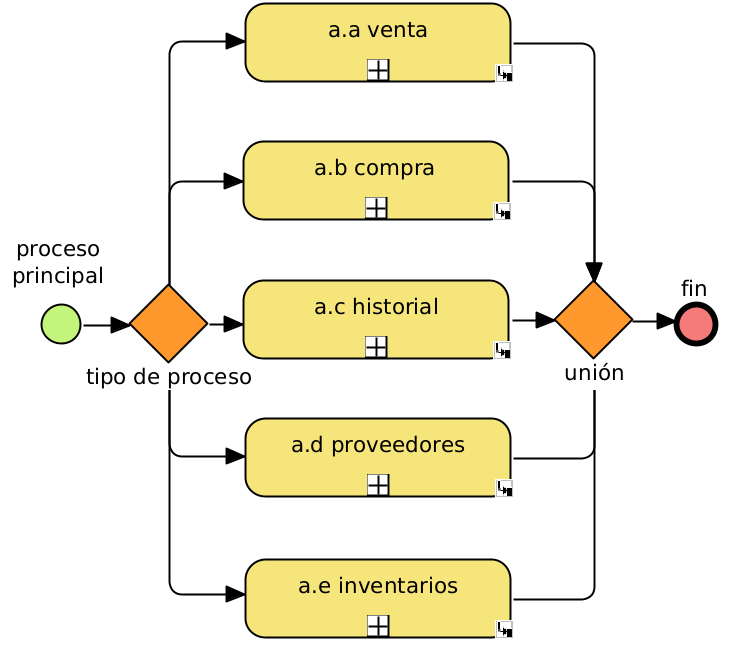
\includegraphics[width=8cm]{proceso/images/a.main.png}\\	

		\normalsize{El diagrama representa los procesos principales que engloban al negocio}
	\end{center}
	
	%------------------------------------------------------------------------------------------------

	%------------------------------------------------------------------------------------------------
	\subsection{Picinas principales}
	 
	\begin{center}
	
	% Referencia al diagrama
	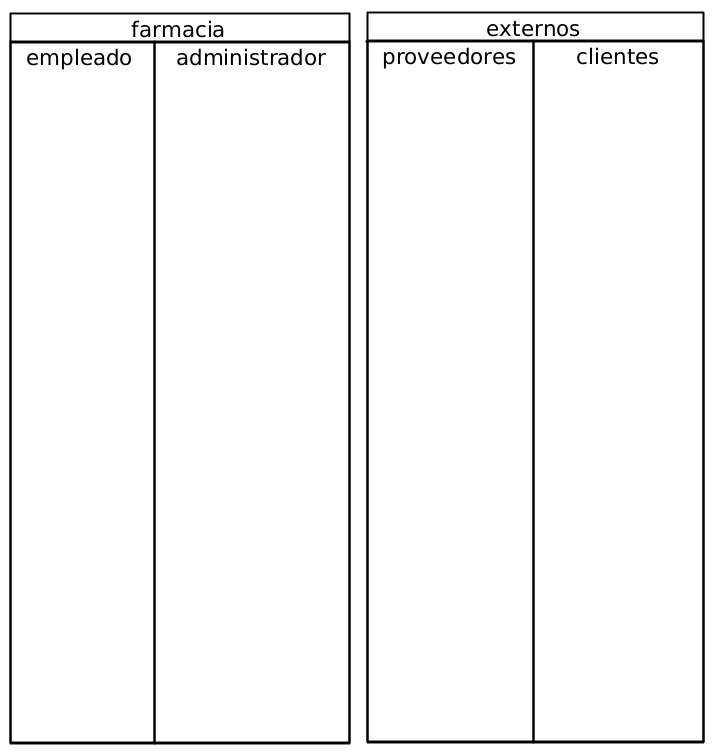
\includegraphics[width=8cm]{proceso/images/a.pools.png}\\	
	
	\normalsize{El diagrama representa las picinas principales del BPMN}
	\end{center}
		
	%------------------------------------------------------------------------------------------------

	%------------------------------------------------------------------------------------------------
	\subsection{Venta}
	 
	\begin{center}
	
	% Referencia al diagrama
	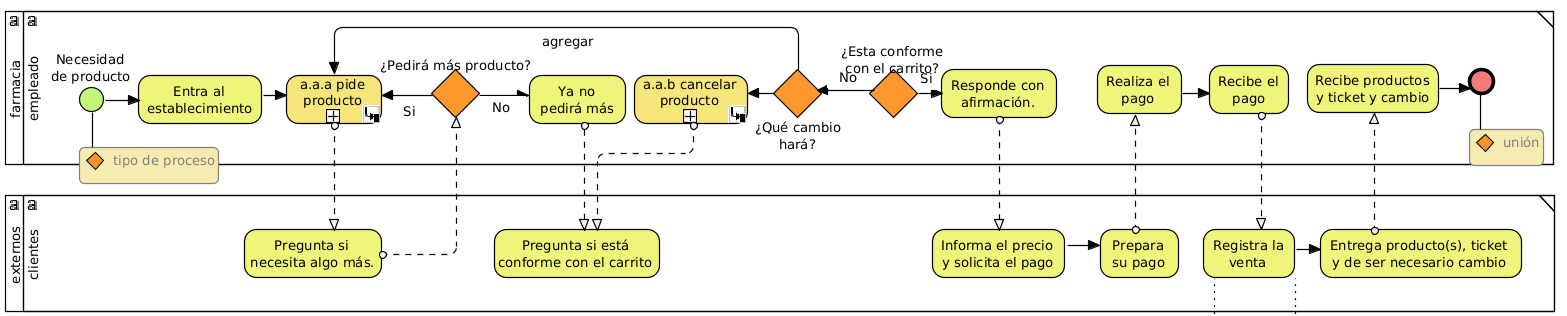
\includegraphics[width=14cm]{proceso/images/a.a.venta.png}\\	
	
	\normalsize{El diagrama representa el proceso relacionado a la venta del cliente}
	\end{center}
		
	%------------------------------------------------------------------------------------------------

	%------------------------------------------------------------------------------------------------
	\subsection{Compra}
	 
	\begin{center}
	
	% Referencia al diagrama
	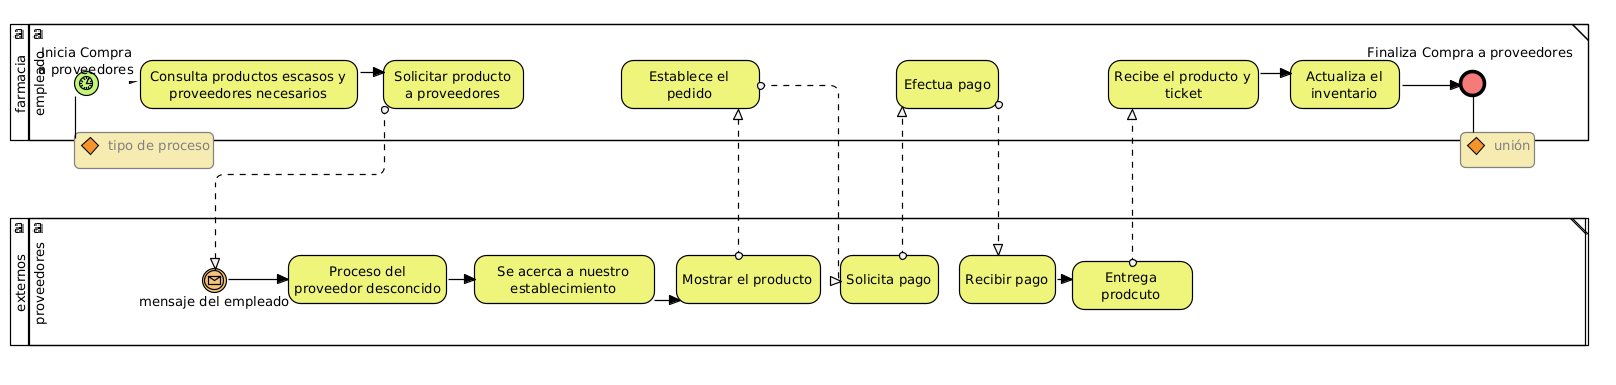
\includegraphics[width=14cm]{proceso/images/a.b.compra.png}\\	
	
	\normalsize{El diagrama representa el proceso relacionado a la compra al proveedor}
	\end{center}
		
	%------------------------------------------------------------------------------------------------

	%------------------------------------------------------------------------------------------------
	\subsection{Proveedores}
	 
	\begin{center}
	
	% Referencia al diagrama
	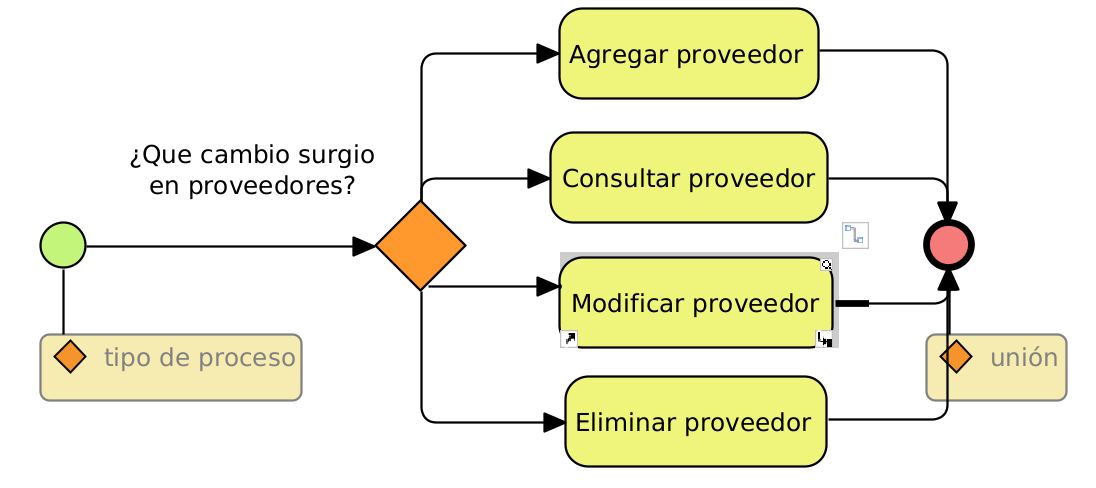
\includegraphics[width=14cm]{proceso/images/a.d.proveedores.png}\\	
	
	\normalsize{El diagrama representa el proceso relacionado al proveedor}
	\end{center}
		
	%------------------------------------------------------------------------------------------------

	%------------------------------------------------------------------------------------------------
	\subsection{Inventario}
	 
	\begin{center}
	
	% Referencia al diagrama
	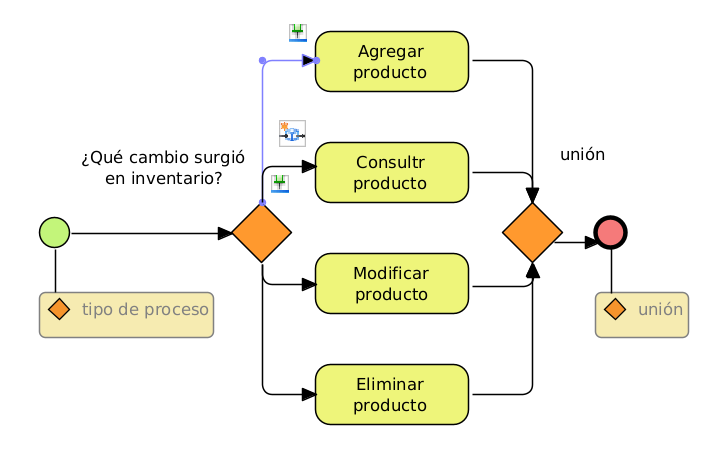
\includegraphics[width=14cm]{proceso/images/a.e.inventario.png}\\	
	
	\normalsize{El diagrama representa el proceso relacionado al inventario}
	\end{center}
		
	%------------------------------------------------------------------------------------------------

	\newpage
	\section{Casos de uso}
	
	\subsection{Diagrama de casos de uso}
	\begin{center}

		% Referencia al diagrama
		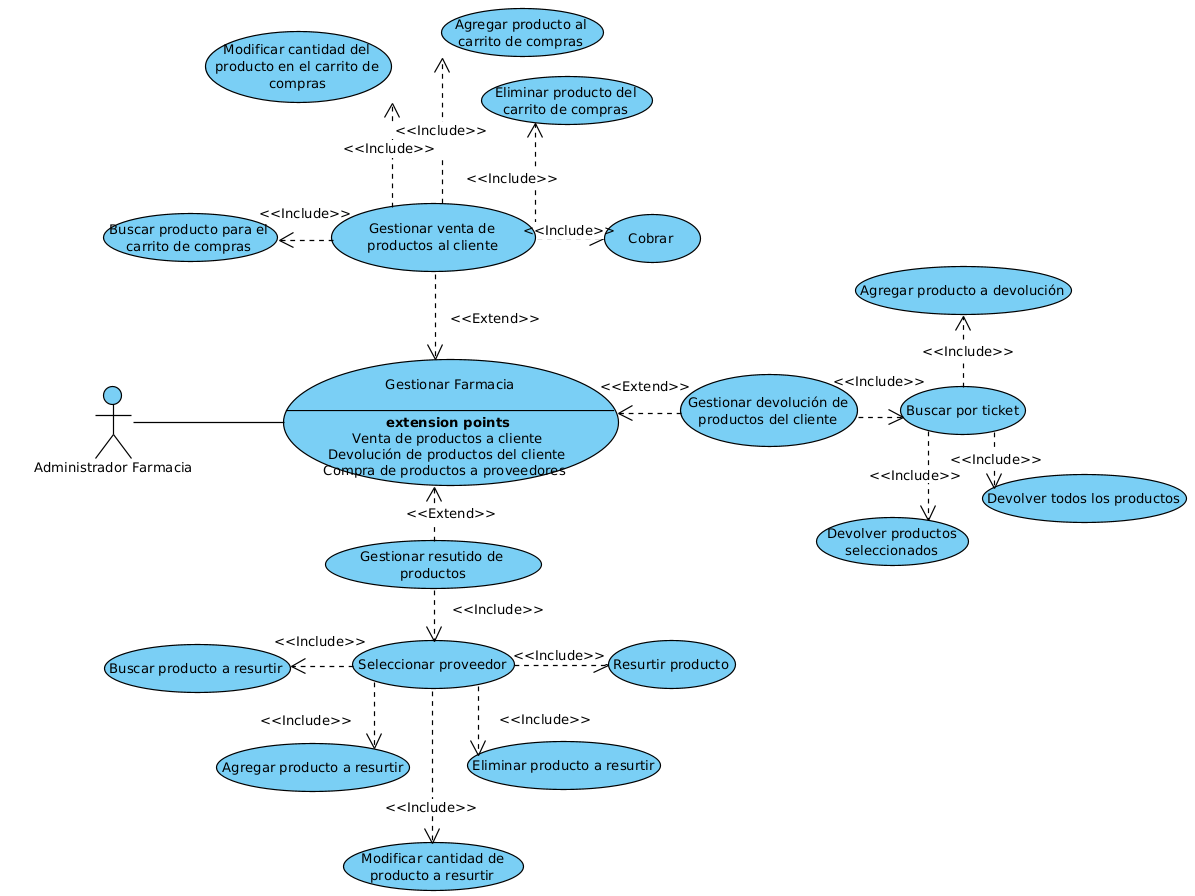
\includegraphics[width=16cm]{proceso/images/x.casosuso.png}\\	

		\normalsize{El diagrama representa los casos de uso derivados del proceso}
	\end{center}
	
	%------------------------------------------------------------------------------------------------

\end{flushleft}